Nesta seção será descrito o diagrama de máquina de estados, presente no SysML e também no UML. Ele é um diagrama comportamental que apresenta as interações entre sistemas ou partes do sistema.

%\subsubsection{O que é o diagrama de sequência}
%Texto

\subsubsection{Estrutura dos diagramas de sequência}
\begin{figure}[H]
\centering
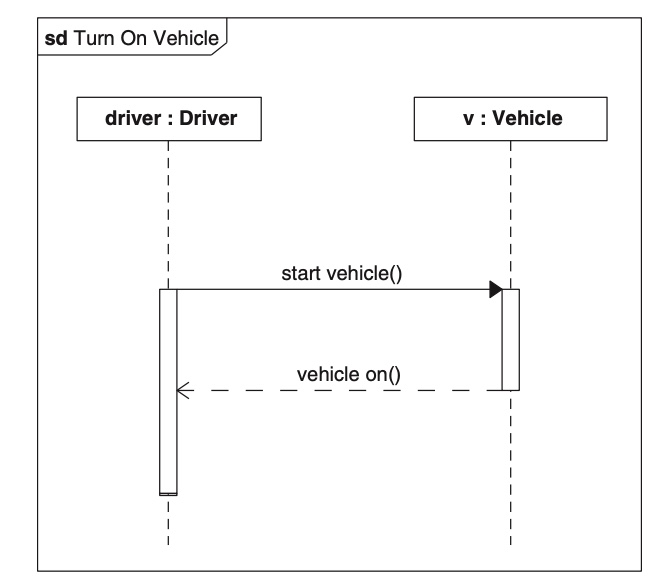
\includegraphics[width=0.75\textwidth]{figures/diagrama-sequencia.jpeg}
\caption{Diagrama de Sequência}
\label{fig:sequence_diagram}
\end{figure}
Representa as interações entre cada parte do sistema, sendo que cada parte é representada por um bloco com o nome dessa parte, cada uma possui uma linha vertical representando o tempo de vida de cada subparte durante certa interação. Na figura \ref{fig:sequence_diagram}, temos o \textit{Driver} e o \textit{Vehicle} sendo apresentados, junto com o tempo de vida de cada um. 

Pode-se indicar interações que ocorrem simultaneamente ou ainda intereações alternativas, dependendo de alguma condição apresentada. Também mostra-se nesse diagrama a troca de mensagens. 

Essa última é indicada pela utilização de setas, sendo que podem-se tratar-se de mensagens síncronas, onde espera-se uma resposta, ou mensagens assíncronas, caso contrário. Também utiliza-se uma seta diferente para representar uma resposta a uma mensagem síncrona. Na figura \ref{fig:sequence_diagram}, pode-se observar o envio da mensagem de iniciar o veículo por parte do \textit{Driver}, e a resposta do \textit{Vehicle} indicando que está ligado.

\subsubsection{Onde são utilizados com frequência}
Utilizado principalmente para representar a interação entre diferentes objetos em um determinado caso de uso, geralmente é criado nos estágios iniciais do desenvolvimento devido á sua capacidade de representar os aspectos dinâmicos do sistema, além de permitir uma revisão nos casos de uso durante a construção desse.

Além de ser usado para definir o funcionamento de determinada funcionalidade antes da implementação dessa, é útil ainda para auxiliar na compreensão de alguma já existente, caso já exista esse diagrama e ele esteja atualizado com o estado do sistema em determinado momento.